\chapter{Resultados}

\section{Simulaciones}

\subsection{Descriptiva}


\begin{figure}[H]
\centering
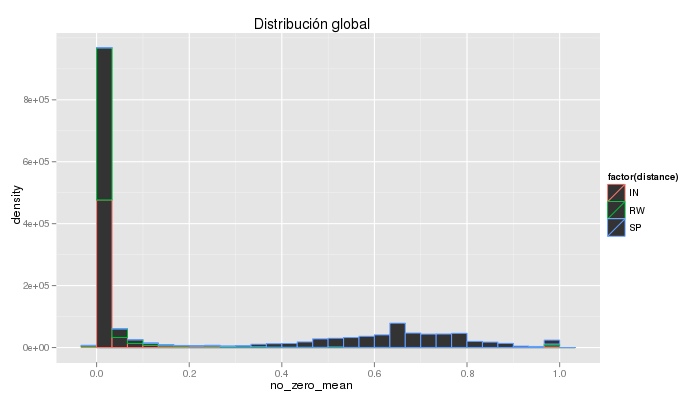
\includegraphics[scale=0.45]{images/emp_tabla_global.png} 
\caption{Distribución global de los estadísticos de priorización obtenidos para el total de simulaciones. La distribución muestra claramente comportamientos muy distintos entre las medidas de distancia planteadas.}
\label{fig:emp_global}
\end{figure}

\medskip
\medskip

\begin{figure}[H]
\centering
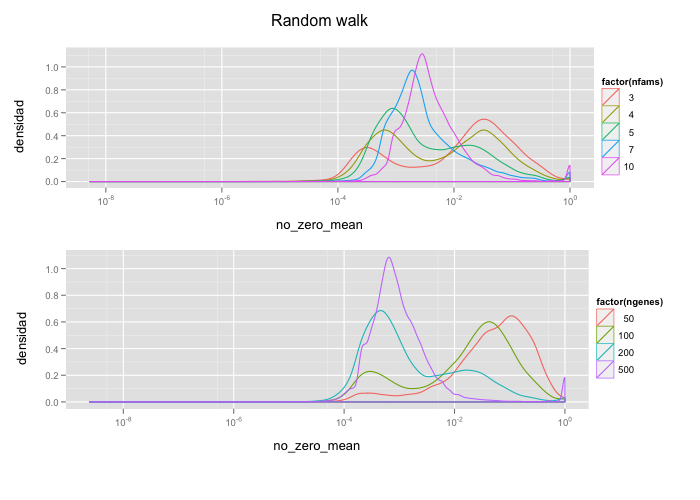
\includegraphics[scale=0.45]{images/emp_rw_nfams_ngenes.png} 
\caption{Distribución global del estadístico de priorización para diferente número de familias (arriba) y diferente número de genes por familia (abajo)..}
\label{fig:emp_rw_nfams_ngenes}
\end{figure}

\medskip
\medskip
 
\subsection{Eficacia en la priorización}

En este apartado, se detallan los resultados obtenidos en las distintas tandas de simulación generadas con el fin de evaluar tanto las medidas de distancia, como la influencia de los parámetros \emph{número de familias}, \emph{número de genes por familia} y \emph{número de genes de enfermedad} sobre los resultados. 

\medskip
Hay que destacar, que en la mayor parte de ocasiones, la fiabilidad de la metodología se ha evaluado a partir de la posición relativa en el ranking de los genes de enfermedad, donde un valor próximo a 1 indicará que han sido convenientemente priorizados por encima del resto de genes aleatorios y que por tanto, la metodología propuesta es efectiva.

\subsubsection{Medidas de distancia}

Las medidas de distancia propuestas han sido evaluadas a partir de las tandas de simulación descritas en la tabla \ref{tab:tabla_distancias} del apartado de material y métodos. Los resultados obtenidos se muestran en la figura \ref{fig:distancias}, la cual representa la posición relativa en el ranking para los genes de enfermedad en las 3 medidas de distancia (\emph{Shortest Path}, intermediación y \emph{Random Walk}) y en los 5 interactomas seleccionados (\emph{binding, functional, ptmod, regulation y textmining}). 

\medskip
Además, se han incluido dos medidas adicionales (\emph{no zero mean} y \emph{no zero max}) correspondientes a las dos funciones propuestas (media y máximo) para proporcionar una medida conjunta de todos los interactomas. Asímismo, las gráficas se han complementado con una barra (de color amarillo) en cada medida, correspondiente a la proporción de genes analizados que no presentan ninguna interacción descrita, y que, por tanto, no han podido ser evaluados en el interactoma correspondiente. 

\begin{figure}[H]
\centering
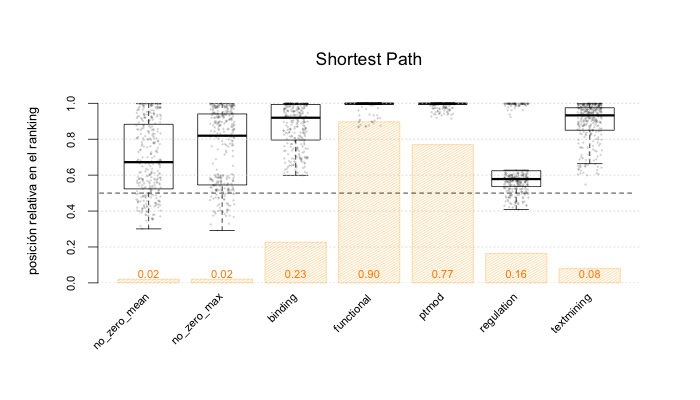
\includegraphics[scale=0.45]{images/sp_summary.png}
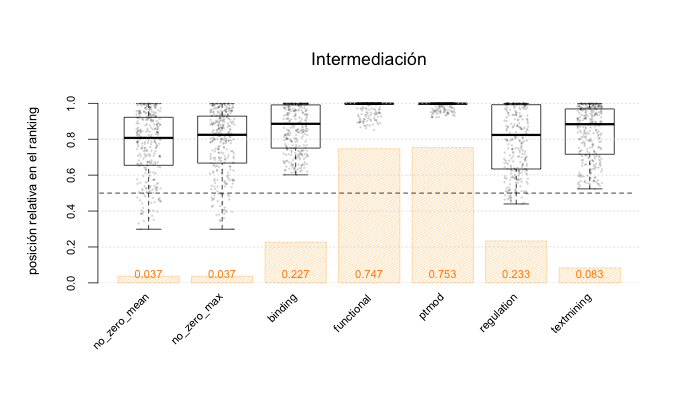
\includegraphics[scale=0.45]{images/inter_summary.png}
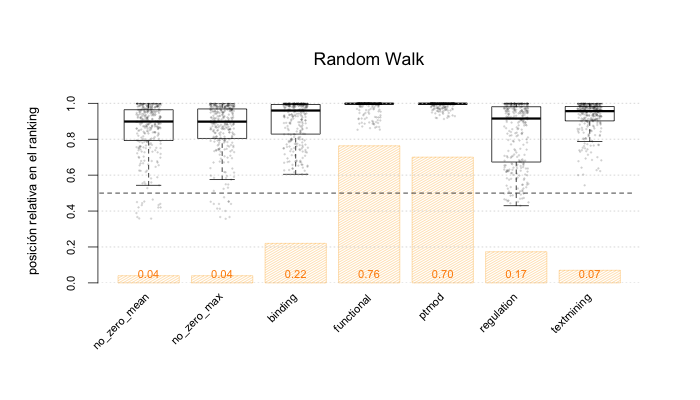
\includegraphics[scale=0.45]{images/rw_summary.png}
\caption{Distribución de la posición relativa en el ranking de los genes de enfermedad para cada medida de distancia \emph{Shortest Path}, intermediación y \emph{Random walk} y cada interactoma. Las barras en amarillo bajo cada interactoma describen la proporción de genes que no han tenido ninguna interacción descrita}
\label{fig:distancias}
\end{figure}

\medskip
Las gráficas describen con claridad como el método \emph{Random walk} proporciona la mejor posición relativa en el ranking para los genes de enfermedad, siendo una mejora perceptible tanto en las medidas por interactoma, como en las medidas globales. Asímismo, se observa que la medida de distancia de intermediación resulta superior a la de \emph{Shortest Path} en todos los casos.

\medskip
En cuanto a los resultados obtenidos por interactoma, se observa claramente que tanto el interactoma funcional, como el de modificaciones post-transduccionales (\emph{functional} y \emph{ptmod} respectivamente) proporcionan con diferencia los mejores resultados, pero también, un porcentaje de genes no descritos muy superior al resto. 

\medskip
A excepción de la medida de distancia \emph{Shortest Path}, tanto la media como el máximo global proporcionan resultados muy similares. Hay que destacar que, salvo el interactoma de regulación, ambas medidas proporcionan un valor de posición en el ranking inferior al de los interactomas, aunque, con un porcentaje de genes no descritos muy inferior al resto.

\subsubsection{Número de familias}

La tabla \ref{tab:tabla_familias} muestra el conjunto de simulaciones planteados para evaluar la influencia del número de familias sobre el resultado. La figura \ref{fig:familias} muestra la distribución de la posición relativa en el ranking para los genes de enfermedad para las 3 medidas de distancia, donde se han usado 3,4,5,7 y 10 familias respectivamente. 

\begin{figure}[H]
\centering
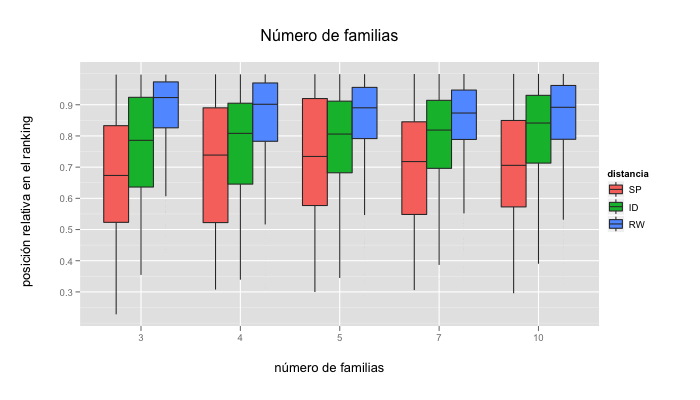
\includegraphics[scale=0.5]{images/tabla_familias.png}
\caption{Distribución de la posición relativa del ranking de los genes de enfermedad para cada número de familias y cada medida de distancia}
\label{fig:familias}
\end{figure}

\medskip
En general, el número de familias no constituye un parámetro que modifique la fiabilidad del resultado. Todas las medidas de distancias muestran  medianas parecidas con dispersión casi constante, siendo la medida de \emph{Shortest Path} la más inestable.
 

\subsubsection{Número de genes por familia}

El número de genes por familia se ha evaluado a partir de las simulaciones planteadas en la tabla \ref{tab:tabla_genes}. La figura \ref{fig:genes} muestra la evolución de la posición relativa en el ranking en función del número de genes por familia.

\begin{figure}[H]
\centering
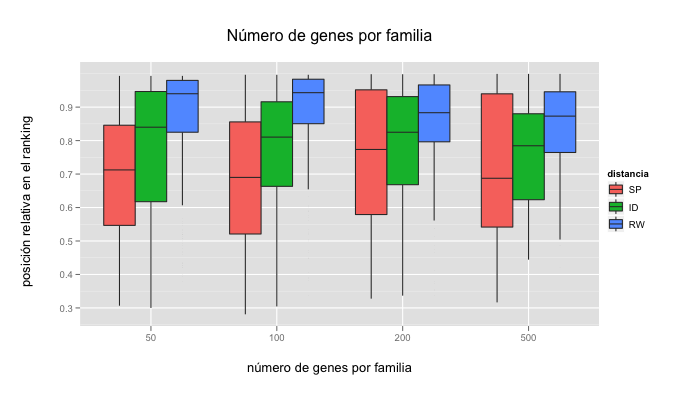
\includegraphics[scale=0.5]{images/tabla_genes.png}
\caption{*****}
\label{fig:genes} 
\end{figure}

\medskip
También en este caso, la medida de \emph{Shortest Path} muestra un comportamiento irregular. Por otro lado, tanto en la distancia de intermediación, como con \emph{Random walk} se aprecia una ligera tendencia decreciente de la mediana, a medida que aumenta el número de genes por familia, con una dispersión casi constante.

\subsubsection{Solapamiento entre familias}

El solapamiento entre familias a nivel de genes de enfermedad se ha evaluado a través de los experimentos planteados en la tabla \ref{tab:tabla_disease}. Todas las simulación se han realizado con 5 familias, donde el número de genes de enfermedad ha estado en el rango de 1 a 5. 

\medskip
La figura \ref{fig:disease} muestra la variación de la posición relativa en el ranking a medida que aumenta el número de genes distintos de enfermedad.

\begin{figure}[H]
\centering
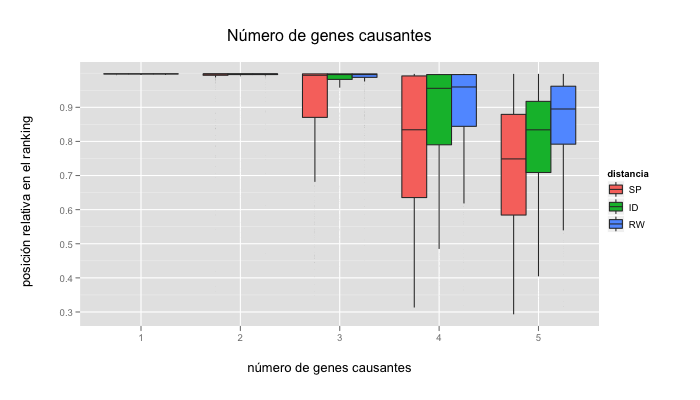
\includegraphics[scale=0.5]{images/tabla_disease.png}
\caption{*****}
\label{fig:disease} 
\end{figure}

\medskip
Tal y como se aprecia, el número de genes de enfermedad distintos tiene una influencia clara sobre el resultado. En aquellos casos donde el número de genes distintos es pequeño, y por tanto, hay gran solapamiento entre familias, se obtienen resultados considerablemente mejores para cualquiera de las medidas de distancia. 

\medskip
También en este caso, \emph{Randow Walk }ofrece los mejores resultados, seguido de la distancia de intermediación.

\section{Caso de uso}
